\documentclass[../main.tex]{subfiles}
\usepackage{slashed}
\usepackage[table]{xcolor}
\usepackage{hhline}
\usepackage{lipsum}

\let\Bbbk\relax
\usepackage{amsmath}
\usepackage{amsfonts}
\usepackage{simpler-wick}

\begin{document}
%\setchapterstyle{kao} % decommentare se non si mette l'immagine
\setchapterimage[6.5cm]{images_ch7/QFT_inf.jpg}
\setchapterpreamble[u]{\margintoc}
\chapter[Dalle Particelle ai Campi]{Dalle Particelle ai Campi\footnote{Immagine da \href{https://www.quantamagazine.org/the-mystery-at-the-heart-of-physics-that-only-math-can-solve-20210610/}{The Mystery at the Heart of Physics That Only Math Can Solve
}.}}
%\labch{pcles_to_fields}
\label{ch:pcles_to_fields}
\fboxsep =1pt % separazione per i box

\section{Operatore di Scattering e Proprietà delle Interazioni}
Torniamo alla situazione che abbiamo delineato all'inizio del capitolo \ref{ch:spacetime_symm}:
\[
|\psi\rangle \xrightarrow[]{ H_\text{int}} |\varphi\rangle 
\]

Ora sappiamo come caratterizzare gli stati multi-particellari \(|\psi\rangle\) e sappiamo anche che tali stati trasformano secondo rappresentazioni unitarie irriducibili del gruppo di Poincaré, in accordo con il teorema di Wigner.

Tuttavia, supponendo di voler studiare un esperimento di scattering, siamo interessati alla situazione in cui pacchetti di particelle si avvicinano tra loro partendo da una distanza macroscopicamente grande, che successivamente interagiscono in una regione microscopicamente piccola e che si allontanano fino a trovarsi nuovamente ad una distanza macroscopicamente grande.

Gli stati prima e dopo l'interazione sono assimilabili a stati di particella libera, precisamente i nostri stati multi-particellari \(|\psi\rangle\).

In questo caso, il prodotto scalare a cui siamo interessati non è della forma \(\langle\varphi|\psi\rangle\), ma piuttosto del tipo:
\[
S_{fi} = \langle f| U(+\infty, -\infty) |i\rangle
\]

L'interpretazione di questo bra-ket è la seguente:
\begin{itemize}
    \item Prendiamo uno stato multi-particellare $|i\rangle$ ad un certo tempo $t\rightarrow -\infty$.
    \item Lo evolviamo per mezzo dell'operatore $U(+\infty, -\infty)$ fino allo stato finale al tempo $t\rightarrow +\infty$.
    \item Calcoliamo l'overlap tra lo stato evoluto e lo stato finale di interesse $|f\rangle$.
\end{itemize}

Consideriamo i casi in cui l'Hamiltoniana è separata in una parte “libera” ed una di “interazione”. Sostanzialmente stiamo considerando la Rappresentazione di Interazione di Dirac, in cui l'evoluzione temporale è dettata dall'Hamiltoniana \(\hat{H} = \hat{H}_0+\hat{H}_\text{int}\) e secondo cui gli operatori evolvono con l'Hamiltoniana libera $\hat{H}_0$, mentre gli stati evolvono con l'Hamiltoniana di interazione $\hat{H}_\text{int}$.

In questa rappresentazione, l'operatore di evoluzione è il ben noto operatore di scattering (o matrice $\pazocal S$), espressa per mezzo della serie di Dyson:

\[
\boxed{U_I(\infty, -\infty) \equiv \pazocal S = \sum_{n=0}^\infty \frac{(-i)^n}{n!}\int_{}d^4x_1\cdots d^4x_n T[\hat{H}^I_\text{int}(x_1)\cdots \hat{H}^I_\text{int}(x_n)]}
\]
Siccome vogliamo che $S_{fi}$ sia invariante sotto trasformazioni di Poincaré, per \(U(\Lambda, a)\in\pazocal P \equiv ISO^+(1,3)\), troviamo:
\[
\langle f| \pazocal S |i\rangle \overset{!}{=} \langle f| U(\Lambda, a)^\dagger\pazocal S U(\Lambda, a) |i \rangle
\]

Ma questo implica \(U(\Lambda, a)^\dagger\pazocal S U(\Lambda, a) {=} \pazocal S\), ovvero:
\[
\pazocal S U(\Lambda, a) {=} U(\Lambda, a)\pazocal S \Rightarrow \boxed{\big[S, U(\Lambda,a)\big] = 0}
\]
Quindi, \textbf{per ottenere l'invarianza relativistica nella nostra teoria, la matrice $\pazocal S$ deve commutare con l'operatore} $U(\Lambda,a)$ \textbf{che adopera le trasformazioni di Poincaré sugli stati di particella libera}. Questa condizione produce interessanti vincoli sull'Hamiltoniana di interazione, in quanto l'invarianza di $\pazocal S$ segue direttamente se si considera $\hat{H}^I_\text{int}(x)$ t.c.:

\begin{equation}
    \boxed{
    \begin{aligned}
        &U(\Lambda, a) \hat{H}^I_\text{int}(x) U(\Lambda, a)^{-1} = \hat{H}^I_\text{int}(\Lambda x + a)\\
        &\big[\hat{H}^I_\text{int}(x),\hat{H}^I_\text{int}(y)\big] = 0\quad \text{se } (x-y)^2<0 
    \end{aligned}}
    \label{eq:hamilt_requirements}
\end{equation}

Se ignoriamo l'ordinamento temporale $T[\cdots]$, la tesi è dimostrata in un passaggio:
\begin{align*}
    U(\Lambda, a) \pazocal S U(\Lambda, a)^{-1} &= \sum_{n=0}^\infty \frac{(-i)^n}{n!}\int_{}d^4x_1\cdots d^4x_n [\hat{H}^I_\text{int}(\Lambda x_1 + a)\cdots \hat{H}^I_\text{int}(\Lambda x_n + a)]
\end{align*}
Da qui con un cambio di variabile $\Lambda x_i + a \equiv y_i$ abbiamo finito, la misura di integrazione $d^4x$ è invariante (essendo il Jacobiano che figura nel cambio di variabile il determinante di $\Lambda$, che è 1) ergo abbiamo \(U(\Lambda, a) \pazocal S U(\Lambda, a)^{-1} = \pazocal S\).

Chiaramente, trascurare il time-ordering è un'approssimazione bella grossa. La logica di fondo è la stessa, ma tenendone conto emerge una situazione interessante, che giustifica la richiesta di commutazione tra gli operatori Hamiltoniani quando calcolati in punti separati da un intervallo di tipo spazio (fuori dal cono di luce).

Nel caso di $n=2$, $U(\Lambda, a) \pazocal S U(\Lambda, a)^{-1}$ assume la seguente struttura:
\[
\begin{aligned}
    \int_{}d^4x_1 d^4x_2 \big[&\Theta(x^0_1-x^0_2)\hat{H}^I_\text{int}(\Lambda x_1 + a)\hat{H}^I_\text{int}(\Lambda x_2 + a) \\
    &+ \Theta(x^0_2-x^0_1)\hat{H}^I_\text{int}(\Lambda x_2 + a)\hat{H}^I_\text{int}(\Lambda x_1 + a)\big]
\end{aligned}
\]
Se ora cambiamo variabile prendendo $\Lambda x_i + a \equiv y_i$ ovvero $x_i \equiv \Lambda^{-1}y_i - \Lambda^{-1}a$, ci troviamo circa nella situazione precedente. Il punto delicato si trova nel fatto che \textbf{la trasformazione di Lorentz implicata dal cambio di variabile potrebbe modificare il segno dell'intervallo temporale} presente nella $\Theta$ di Heaviside.

Quando abbiamo classificato le orbite del gruppo di Poincaré, abbiamo evidenziato e giustificato (in maniera intuitiva) il fatto che ciò non sia possibile nel caso in cui due punti $x_i$ ed $x_j$ siano all'interno del cono di luce, i.e. quando $(x_i-x_j)^2\geq 0$. Il problema evidenziato si verifica dunque solo quando $(x_i-x_j)^2< 0$ ed in tal caso imponiamo che la relazione di commutazione anticipata poc'anzi, \(\big[\hat{H}^I_\text{int}(x),\hat{H}^I_\text{int}(y)\big] = 0\).

Inoltre, siccome vogliamo che l'evoluzione temporale goda della proprietà di unitarietà, $\hat{H}^I_\text{int}(x)$ deve essere anche Hermitiana.

\textbf{Come facciamo a costruire delle Hamiltoniane che abbiano esattamente queste caratteristiche?} Supponiamo di avere due operatori $\hat{O}_{1,2}(x)$ che verifichino individualmente le condizioni (\ref{eq:hamilt_requirements}), i.e.:
\[
\begin{aligned}
    &U(\Lambda, a) \hat{O}_i(x) U(\Lambda, a)^{-1} = \hat{O}_i(\Lambda x + a)~,\quad i=1,2\\
    &\big[\hat{O}_i(x),\hat{O}_j(y)\big] = 0~,\quad \forall~i,j\quad \text{se } (x-y)^2<0 
\end{aligned}
\]
\begin{itemize}
    \item La prima condizione ci dice che gli $\hat{O}_{i}(x)$ sono operatori scalari, ovvero trasformano in maniera banale sotto trasformazioni di Lorentz\footnote{Nel senso che la trasformazione modifica solo la dipendenza spazio-temporale e non la struttura dell'operatore stesso.}.
    \item La seconda condizione è detta di micro-causalità.
    \begin{theorem}
        \textbf{(Condizione di Micro-causalità.)}

        Due osservabili misurati in due punti spazio-temporali connessi da un intervallo di tipo spazio devono commutare tra loro.
        \label{th:microcausality}
    \end{theorem}
    Due osservabili mutualmente commutanti possono essere misurati in contemporanea senza che le due misure interferiscano tra loro, i.e. non sono in contatto causale.
\end{itemize}
A questo punto ci sono due fatti notevoli, e facili da dimostrare:
\begin{enumerate}
    \item[\textbf{(i.)}] Il prodotto $\hat{O}(x) = \hat{O}_{1}(x)\hat{O}_{2}(x)$ è ancora un operatore scalare.
    \item[\textbf{(ii.)}] Considerando $\hat{O}(\cdot)$ in due punti separati da un intervallo di tipo spazio la condizione di micro-causalità è ancora valida.
\end{enumerate}
Appare quindi chiaro quale sia l'opzione più semplice per costruire gli operatori Hamiltoniani che ci interessano: sfruttare il prodotto di \textbf{operatori di campo scalari}\marginnote{Indichiamo con operatore di campo scalare un operatore agente su uno stato multi-particellare}, tutti valutati nello stesso punto $x\in\mathbb M^4$.

Per quanto il termine sia nuovo, abbiamo già incontrato degli oggetti che si identificano con gli operatori di campo scalari: \textbf{gli operatori di creazione e distruzione}!

\section{Campi Scalari}
\subsection{Il campo scalare neutro}
La combinazione più semplice che possiamo costruire a partire dagli operatori di creazione e distruzione è il cosiddetto campo scalare neutro:\marginnote{Gli operatori di creazione e distruzione nascondono al loro interno anche la massa del campo, nel caso in cui questo ne sia dotato.}
\begin{equation}
    \begin{aligned}
        &\boxed{\hat{\Phi}(x) = \int_{}\frac{d^3\Vec{p}}{(2\pi)^3\sqrt{2p^0}}\big[ a(\Vec{p})e^{-ip\cdot x} + a^\dagger(\Vec{p})e^{ip\cdot x} \big]}\\
        &\hat{\Phi}(x)^\dagger = \hat{\Phi}(x) ~;\quad p^0=+E_{\Vec{p}} 
    \end{aligned}
    \label{eq:neutral_scalar_field}
\end{equation}
Riguardo l'equazione (\ref{eq:neutral_scalar_field}) possiamo fare i seguenti commenti:
\begin{enumerate}
    \item[\textbf{1)}] La presenza dei fattori \(e^{\pm ip\cdot x}\) rende il campo automaticamente compatibile con la proprietà di trasformazione sotto traslazioni in $\mathbb M^4$. Si verifica infatti, senza troppa difficoltà, per mezzo delle proprietà di trasformazione di $a(\Vec{p})$ e $a^\dagger(\Vec{p})$, rispettivamente eq. (\ref{eq:creation_operators_underpoincare}) e (\ref{eq:annihil_operators_underpoincare}) considerate nel caso in cui $\Lambda = \mathbb 1$, che:
    \[
    U(\mathbb 1, a)\hat{\Phi}(x) U(\mathbb 1, a)^{-1} \overset{!}{=} \hat{\Phi}(x + a)
    \]
    \item[\textbf{2)}] Gli operatori $a(\Vec{p})$ e $a^\dagger(\Vec{p})$ creano ed annichiliscono stati scalari (ovvero senza spin) e sotto trasformazione di Lorentz si può verificare che:
    \[
    U(\Lambda, 0)\hat{\Phi}(x) U(\Lambda, 0)^{-1} \overset{!}{=} \hat{\Phi}(\Lambda x)
    \]
    \begin{proof}
    Siccome qui la situazione è un po' più subdola, è opportuno svolgere questo conto nel dettaglio. Innanzitutto possiamo riscrivere, preso  $U(\Lambda, 0) \equiv  U(\Lambda)$ ed applicando le regole di trasformazione di $a^{(\dagger)}(\Vec{p})$ nel caso di stati spinless:

    \begin{align*}
        U(\Lambda)\hat{\Phi}(x) U(\Lambda)^{-1} &= \int_{}\frac{d^3\Vec{p}}{(2\pi)^3\sqrt{2p^0}} \sqrt{\frac{(\Lambda p^0)}{p^0}}\big[ a(\Vec{p})e^{-ip\cdot \Lambda x} + a^\dagger(\Vec{p})e^{ip\cdot \Lambda x} \big] \\
        \hat{\Phi}(\Lambda x) &= \int_{}\frac{d^3\Vec{p}}{(2\pi)^3\sqrt{2p^0}} \big[ a(\Vec{p})e^{-ip\cdot \Lambda x} + a^\dagger(\Vec{p})e^{ip\cdot \Lambda x} \big]
    \end{align*}

    Ora arriva il trucco che verifica l'uguaglianza tra le due espressioni: lavoriamo su $\hat{\Phi}(\Lambda x)$ e moltiplichiamo e dividiamo per $\sqrt{p^0}$, accorpando le due $\sqrt{p^0}$ a denominatore, così da ottenere un fattore $\nicefrac{d^3\Vec{p}}{p^0}$, che è invariante sotto trasformazione di Lorentz.
    \marginnote{\textbf{Attenzione:} Qui stiamo introducendo una procedura che utilizzeremo più volte nel seguito, ed a cui, per comodità di notazione, ci riferiremo sempre come “cambio di variabile ...”, sottintendendo gli altri passaggi elencati prima e dopo.}
    Se successivamente \textbf{adottiamo il cambio di variabile} $p^\mu \rightarrow \Lambda p^\mu$ (che implica $\Vec{p}\rightarrow \Vec{p}_\Lambda$ e $p^0\rightarrow(\Lambda p)^0$) arriviamo alla seguente espressione: 
    \begin{align*}
        \hat{\Phi}(\Lambda x) &= \int_{}\frac{d^3\Vec{p}}{(2\pi)^3\sqrt{2}p^0} \sqrt{(\Lambda p)^0}\big[ a(\Vec{p})e^{-i\Lambda p\cdot \Lambda x} + a^\dagger(\Vec{p})e^{i\Lambda p\cdot \Lambda x} \big]
    \end{align*}
    Il gioco è dunque fatto, possiamo separare $p^0 = \sqrt{p^0}\sqrt{p^0}$ e sfruttare l'invarianza del prodotto scalare sotto trasformazione di Lorentz e l'uguaglianza è verificata.
    \end{proof}
    
    \item[\textbf{3)}] Gli operatori $a(\Vec{p})$ e $a^\dagger(\Vec{p})$ appaiono con gli stessi fattori di proporzionalità, e questo porta alla verifica della condizione di micro-causalità. 
    
    La verifica è banale se si ricorda che tra gli operatori di creazione e distruzione vigono le seguenti relazioni di commutazione:
    \begin{equation}
        \boxed{
        \begin{aligned}
            \big[ a(\Vec{p}), a(\Vec{k}) \big] &= \big[ a^\dagger(\Vec{p}), a^\dagger(\Vec{k}) \big] = 0\\
            \big[a(\Vec{p}), a^\dagger(\Vec{k}) \big] &= (2\pi)^3\delta(\Vec{p}-\Vec{k})
        \end{aligned}
        }
        \label{eq:creat_annihl_comm_rel}
    \end{equation}
    Se ad esempio ci fosse stato un fattore \(\frac{1}{2}\) di fronte a solo uno dei due la condizione sarebbe invalidata.
\end{enumerate}

\subsection{Il campo scalare carico}
Discutiamo ora una possibile generalizzazione del campo scalare neutro, introducendo il campo scalare carico, per cui non vale la condizione di Hermitianietà, i.e. $\hat{\Phi}(x)^\dagger \neq \hat{\Phi}(x)$.

Tale operatore ha la seguente forma:
\begin{equation}
    \boxed{\begin{aligned}
        &\hat{\Phi}(x) = \int_{}\frac{d^3\Vec{p}}{(2\pi)^3\sqrt{2p^0}}\big[ a(\Vec{p})e^{-ip\cdot x} + b^\dagger(\Vec{p})e^{ip\cdot x} \big]\\
        &\hat{\Phi}^\dagger(x) = \int_{}\frac{d^3\Vec{p}}{(2\pi)^3\sqrt{2p^0}}\big[ b(\Vec{p})e^{-ip\cdot x} + a^\dagger(\Vec{p})e^{ip\cdot x} \big]
    \end{aligned}}
    \label{eq:charged_scalar_field}
\end{equation}

Il metodo più semplice per costruire un campo di questo tipo è considerare due campi scalari indipendenti di pari massa $\hat{\Phi}_1(x)$ e $\hat{\Phi}_2(x)$ t.c.:
\begin{align*}
    \hat{\Phi}_i(x) = \int_{}\frac{d^3\Vec{p}}{(2\pi)^3\sqrt{2p^0}}\big[ a_i(\Vec{p})e^{-ip\cdot x} + a_i^\dagger(\Vec{p})e^{ip\cdot x} \big]
\end{align*}
e tra i cui operatori di creazione e distruzione valgono le seguenti relazioni di commutazione:
\begin{align*}
    \big[ a_i(\Vec{p}), a_j(\Vec{k}) \big] &= \big[ a_i^\dagger(\Vec{p}), a_j^\dagger(\Vec{k}) \big] = 0~, \quad \forall~i,j\in[1,2]\\
    \big[a_i(\Vec{p}), a_j^\dagger(\Vec{k}) \big] &= \delta_{ij}(2\pi)^3\delta(\Vec{p}-\Vec{k}) ~,\quad i\neq j
\end{align*}

Possiamo quindi combinare questi due campi definendo:
\begin{align*}
    &\hat{\Phi}(x) = \frac{1}{\sqrt{2}}\big[ \hat{\Phi}_1(x) + i \hat{\Phi}_2(x)\big]\\
    &\hat{\Phi}^\dagger(x) = \frac{1}{\sqrt{2}}\big[ \hat{\Phi}_1(x) - i \hat{\Phi}_2(x)\big]
\end{align*}
Tale definizione genera due tipi di operatori di creazione e distruzione definiti in maniera naturale come segue:


\begin{gather*}
    \textbf{PARTICELLE}\\
    \textbf{Distruzione: }a(\Vec{p}) \equiv \frac{a_1(\Vec{p})+ia_2(\Vec{p})}{\sqrt{2}} ~;\quad 
    \textbf{Creazione: } a^\dagger(\Vec{p}) \equiv \frac{a_1^\dagger(\Vec{p})-ia_2^\dagger(\Vec{p})}{\sqrt{2}}
\end{gather*}

\begin{gather*}
    \textbf{ANTI-PARTICELLE}\\
    \textbf{Distruzione: } b(\Vec{p}) \equiv \frac{a_1(\Vec{p})-ia_2(\Vec{p})}{\sqrt{2}} ~;\quad 
    \textbf{Creazione: } b^\dagger(\Vec{p}) \equiv \frac{a_1^\dagger(\Vec{p})+ia_2^\dagger(\Vec{p})}{\sqrt{2}}
\end{gather*}

Per i quali valgono le seguenti relazioni di commutazione
\begin{align*}
    &\big[ a \text{ o }b, a \text{ o }b \big] = 0\\
    &\big[ a^\dagger \text{ o }b^\dagger, a^\dagger \text{ o }b^\dagger \big] = 0\\
    &\big[a(\Vec{p}), a^\dagger(\Vec{k}) \big] = \big[b(\Vec{p}), b^\dagger(\Vec{k}) \big] =(2\pi)^3\delta(\Vec{p}-\Vec{k})
\end{align*}

Il campo $\hat{\Phi}(x)$ crea una anti-particella tramite $b^\dagger(\Vec{p})$ o annichilisce una particella tramite $a(\Vec{p})$ nella posizione $x$, viceversa per $\hat{\Phi}^\dagger(x)$. La presenza di entrambi i tipi di operatori di creazione e distruzione nei campi è cruciale per garantire la proprietà di micro-causalità. 

Dal punto di vista tecnico, essendo $\hat{\Phi}(x)$ anti-Hermitiano, l'Hamiltoniana (che deve essere Hermitiana) deve contenere sia $\hat{\Phi}$ che $\hat{\Phi}^\dagger$. Questo significa che la micro-causalità è verificata di conseguenza per ogni combinazione possibile. Combinando questa informazione con le relazioni di commutazione degli operatori $a$ e $b$ troviamo:
\[\begin{aligned}
    &\big[ \hat{\Phi}(x),\hat{\Phi}(y) \big] = \big[ \hat{\Phi}^\dagger(x),\hat{\Phi}^\dagger(y) \big] = 0 \quad \forall~x,y\\
    &\big[ \hat{\Phi}(x),\hat{\Phi}^\dagger(y) \big] = \big[ \hat{\Phi}^\dagger(x),\hat{\Phi}(y) \big] = 0 \quad \text{per }(x-y)^2<0
\end{aligned}
\]

\begin{exercise}
    Calcolare esplicitamente $\big[ \hat{\Phi}(x),\hat{\Phi}(y) \big]$ nel caso di un campo scalare reale. \textbf{[Conti svolti Lezione 26p2 pag. 13÷16]}
\end{exercise}

\section{Campi Quantistici di Spin Generico}
Siamo partiti considerando la possibilità più semplice: costruire interazioni tali da rispettare le proprietà (\ref{eq:hamilt_requirements}) per mezzo di prodotti (globalmente Hermitiani) di operatori scalari che rispettino tali proprietà individualmente.

Chiaramente è possibile, seppur più complesso, costruire interazioni tali che $\hat{H}_\text{int}(x)$ sia un oggetto scalare, ma composto da operatori con trasformazioni non banali sotto Lorentz. Ad esempio possiamo considerare il caso in cui l'interazione sia prodotto di un campo 4-vettoriale ed un bilineare di Dirac, i.e.:
\[
\hat{H}_\text{int}(x) = V^\mu(x)\big[\bar\psi(x)\gamma_\mu\psi(x)\big]
\]

in cui la trasformazione del campo quantistico generico $\psi(x)$ è definita secondo \href{https://en.wikipedia.org/wiki/Wightman_axioms#W2_(transformation_law_of_the_field)}{uno degli assiomi di Wightman}:
\begin{equation}
    \boxed{U(\Lambda, a)\psi^a(x)U(\Lambda, a)^{-1} = \sum_b\big[\mathscr D(\Lambda^{-1})\big]^a_{~b}\psi^b(\Lambda x + a)}
    \label{eq:wightman_transform_axiom}
\end{equation}
dove essenzialmente stiamo dicendo che il campo $\psi^a(x)$ trasforma secondo $\mathscr D$, che è una qualche rappresentazione finito-dimensionale del gruppo di Lorentz, tra l'altro non unitaria (in quanto, come già sottolineato dopo l'esempio \ref{example:notbounded_rapidity}, essendo $\pazocal L$ non compatto, non ammette rappresentazioni unitarie finito-dimensionali).

Inoltre il campo $\psi^a(x)$ è definito come segue:
\begin{equation}
    \boxed{
    \psi^a(x) = \sum_\lambda\int_{}\frac{d^3\Vec p}{(2\pi)^3\sqrt{2p^0}}\big[u^a(\Vec{p},\lambda)a(\Vec{p},\lambda,n)e^{-ip\cdot x} + v^a(\Vec{p},\lambda)b^\dagger(\Vec{p},\lambda,n)e^{ip\cdot x}\big]
    }
    \label{eq:generic_quantum_field}
\end{equation}
dove stiamo espandendo l'operatore di campo in funzione degli operatori di creazione e distruzione di tipo “$n$” e per $n$ fissato integriamo e sommiamo sugli stati del multipletto.

\section{Connessione Poincaré - Lorentz}
La domanda cruciale è la seguente: 
\begin{kaobox}
Supponiamo di voler descrivere particelle di tipo “$n$” fissato (diciamo con massa $M$ e spin $s$), secondo quale rappresentazione di Lorentz dovrebbe trasformare $\psi^a(x)$? Questa trasformazione è unica?\footnote{Spoiler: no, non lo è.}
\end{kaobox}
% Vogliamo sostanzialmente “connettere” ciò che abbiamo imparato dalle rappresentazioni irriducibili di $\pazocal P$ alle trasformazioni finito-dimensionali di $\pazocal L$

Per rispondere a questa domanda innanzitutto la formalizziamo dal punto di vista matematico, combinando le equazioni (\ref{eq:wightman_transform_axiom}) e (\ref{eq:generic_quantum_field}), in modo da avere un'equazione da risolvere. Per farlo, utilizzeremo le trasformazioni degli operatori $a(\Vec{p},\lambda,n)$ e $b^\dagger(\Vec{p},\lambda,n)$ sotto Lorentz, che qui riportiamo per comodità:

\begin{align*}
    &\boxed{U(\Lambda)b^\dagger(\Vec{p},\lambda,n)U(\Lambda)^{-1} =\sqrt{\frac{(\Lambda p)^0}{p^0}} \Big[D_s\big(\omega(\Lambda, p)\big)\Big]_{\lambda'\lambda}b^\dagger(\Vec{p}_\Lambda,\lambda',n)}\\
    &U(\Lambda)a(\Vec{p},\lambda,n)U(\Lambda)^{-1} =\sqrt{\frac{(\Lambda p)^0}{p^0}} \Big[D_s\big(\omega(\Lambda, p)\big)\Big]^\ast_{\lambda'\lambda}a(\Vec{p}_\Lambda,\lambda',n)
\end{align*}

Essendo $D_s(\omega)$ unitaria, $D_s(\omega)^\dagger = D_s(\omega)^{-1}$. Possiamo quindi trasporre l'equazione trovando:
\[
D_s(\omega)^\ast = \big[D_s(\omega)^{-1}\big]^{\textcolor{Red}{T}} \Rightarrow \Big[D_s(\omega)\Big]^\ast_{\textcolor{Red}{\lambda'\lambda}} = \Big[D_s(\omega)^{-1}\Big]_{\textcolor{Red}{\lambda\lambda'}} \overset{\text{$D_s$ è rappr.}}{=} \Big[D_s(\omega^{-1})\Big]_{{\lambda\lambda'}}
\]

Possiamo riscrivere l'equazione per $a(\Vec{p},\lambda,n)$ utilizzando l'uguaglianza che abbiamo appena ricavato:
\[
\boxed{U(\Lambda)a(\Vec{p},\lambda,n)U(\Lambda)^{-1} =\sqrt{\frac{(\Lambda p)^0}{p^0}} \Big[D_s\big(\omega(\Lambda, p)^{-1}\big)\Big]_{\lambda\lambda'}a(\Vec{p}_\Lambda,\lambda',n)}
\]

Sostituiamo quindi la (\ref{eq:generic_quantum_field}) nella (\ref{eq:wightman_transform_axiom}) trascurando la traslazione e applichiamo le regole che abbiamo appena visto. Il LHS si riscrive:
\begin{align*}
    U(\Lambda)\psi^a(x)U(\Lambda)^{-1} = \sum_\lambda&\int_{}\frac{d^3\Vec p}{(2\pi)^3\sqrt{2p^0}}\sqrt{\frac{(\Lambda p)^0}{p^0}} \times \\
    \times\Big\{& u^a(\Vec{p},\lambda)e^{-ip\cdot x} \Big[D_s\big(\omega^{-1}\big)\Big]_{\lambda\lambda'} a(\Vec{p}_\Lambda,\lambda',n)\, + \\ 
    &+ v^a(\Vec{p},\lambda)e^{ip\cdot x} \Big[D_s\big(\omega\big)\Big]_{\lambda'\lambda} b^\dagger(\Vec{p}_\Lambda,\lambda',n)\Big\}
\end{align*}

mentre per quanto riguarda il RHS abbiamo:
\begin{align*}
    \big[\mathscr D(\Lambda^{-1})\big]^a_{~b}\psi^b(\Lambda x) = \big[\mathscr D(\Lambda^{-1})\big]^a_{~b}
    \sum_\lambda\int_{}\frac{d^3\Vec p}{(2\pi)^3\sqrt{2p^0}}\big[&u^b(\Vec{p},\lambda)e^{-ip\cdot \Lambda x}a(\Vec{p},\lambda,n) +\\
    &+ v^b(\Vec{p},\lambda)e^{ip\cdot \Lambda x}b^\dagger(\Vec{p},\lambda,n)\big] \overset{\star}{=}
\end{align*}
Adesso adoperiamo il cambio di variabile $p\rightarrow \Lambda p$, come nel caso del campo scalare neutro, e rinominiamo $\lambda \rightarrow \lambda'$, in modo da ottenere:
\begin{align*}
    \overset{\star}{=} \big[\mathscr D(\Lambda^{-1})\big]^a_{~b}
    \sum_{\lambda'}\int_{}\frac{d^3\Vec p_\Lambda}{(2\pi)^3\sqrt{2p^0}}\sqrt{\frac{(\Lambda p)^0}{p^0}}
    \big[&u^b(\Vec{p}_\Lambda,\lambda')e^{-ip\cdot x}a(\Vec{p}_\Lambda,\lambda',n) +\\
    &+ v^b(\Vec{p}_\Lambda,\lambda')e^{ip\cdot x}b^\dagger(\Vec{p}_\Lambda,\lambda',n)\big] 
\end{align*}

Se compariamo LHS ed RHS otteniamo due equazioni, che rappresentano la \textbf{connessione particella-campo} (o Poincaré-Lorentz):\marginnote{Al LHS, con la notazione $\sum_\lambda\big[D_s(\omega)\big]_{\lambda'\lambda}$, stiamo sottintendendo una somma su $\lambda'$, che nel confronto cancella quella del RHS }
\begin{equation}
    \boxed{
    \begin{aligned}
        \sum_\lambda \big[D_s(\omega^{-1})\big]_{\lambda\lambda'} u^a(\Vec{p},\lambda) = 
        \big[\mathscr D(\Lambda^{-1})\big]^a_{~b}u^b(\Vec{p}_\Lambda,\lambda')\\
        \sum_\lambda \big[D_s(\omega)\big]_{\lambda'\lambda} v^a(\Vec{p},\lambda) = \big[\mathscr D(\Lambda^{-1})\big]^a_{~b}v^b(\Vec{p}_\Lambda,\lambda')
    \end{aligned}}
    \label{eq:poinc_lorentz_conn}
\end{equation}
\begin{nota}
    Nel caso massivo, risulta particolarmente utile considerare il problema nella base di polarizzazione di spin, che permette di riscrivere le equazioni come segue \textbf{[conti svolti Lez. 27 pag. 21÷21]}:
    \begin{equation}
        \boxed{
        \begin{aligned}
            \big[\mathscr D(\Lambda)\big]^k_{~n}u^n(\Vec{p},\sigma)= u^k(\Vec{p}_\Lambda,\sigma')\big[D_s(\omega_L)\big]_{\sigma'\sigma}  \\
            \big[\mathscr D(\Lambda)\big]^k_{~n}v^n(\Vec{p},\sigma) = v^k(\Vec{p}_\Lambda,\sigma')\big[D_s(\omega_L)\big]^\ast_{\sigma'\sigma}  
        \end{aligned}}
        \label{eq:poinc_lorentz_conn_spinpol_basis}
    \end{equation}
\end{nota}

\subsection{Strategia della soluzione}
Delineiamo come al solito in maniera schematica le tecniche che useremo in seguito per risolvere questa equazione. La strategia si compone di due step:
\begin{enumerate}
    \item[\textbf{1)}] Consideriamo la prima equazione (riscritta in base di polarizzazione di spin) in $\Vec{p}=0$ e nel caso di $\Lambda = \Lambda_R$ rotazione pura.

    In questo modo possiamo usare il fatto che $\omega_L(\Lambda_R,0) = \Lambda_R$, come enunciato nel teorema \ref{th:wigner_rot_pure_rot}, il che semplifica l'equazione in:
    \begin{equation}
        \boxed{\big[\mathscr D(\Lambda_R)\big]^k_{~n}u^n(\Vec{0},\sigma)= u^k(\Vec{0},\sigma')\big[D_s(\Lambda_R)\big]_{\sigma'\sigma} }
        \label{eq:PL_conn_step1}
    \end{equation}
    che risolta fornisce $u^k(\Vec{0},\sigma)$.
    
    \item[\textbf{2)}] Generalizziamo il risultato del punto \textbf{1)} ad impulso $\Vec{p}$ generico.

    In particolare prendiamo una trasformazione di Lorentz precisamente uguale all'inversa del boost che genera $\Vec{p}$ quando applicata a $\Vec{p}_\text{ref}$, i.e. \(\Lambda = L(\Vec{p},M)^{-1}\).

    La rotazione di Wigner, che ricordiamo essere definita da
    \(\omega_L(\Lambda,p) = L(\Vec{p}_\Lambda,M)^{-1} \Lambda L(\Vec{p},M) \), nel nostro caso corrisponde a:
    \[
    \omega_L(L^{-1},p) = L(\Vec{p}_\Lambda,M)^{-1}
    \]
    Ma c'è di più, poiché in questo caso specifico $\Lambda$ riporta $\Vec{p}$ nel vettore di riferimento $\Vec{p}_\text{ref} =0$, ergo $p_\Lambda = \Vec{0}$! Di conseguenza, dalla definizione di $L(\Vec{p},M)$ (\ref{eq:boost_def_spinpol_basis}):
    \[
    \omega_L(L^{-1},p) = L(\Vec{0},M)^{-1} = \mathbb 1
    \]

    Questo significa che, ripartendo dalla prima equazione delle (\ref{eq:poinc_lorentz_conn_spinpol_basis}) l'equazione diventa:
    \begin{align*}
        \big[\mathscr D\big(L(\Vec{p},M)^{-1}\big)\big]^k_{~n}u^n(\Vec{p},\sigma)&= u^k(\Vec{0},\sigma')\delta_{\sigma'\sigma} \\
        \delta^m_n u^n(\Vec{p},\sigma)&= \big[\mathscr D\big(L(\Vec{p},M)\big)\big]^m_{~k}u^k(\Vec{0},\sigma)
    \end{align*}
    Ovvero:
    \begin{equation}
        \boxed{\big[\mathscr D\big(L(\Vec{p},M)\big)\big]^m_{~k}u^k(\Vec{0},\sigma) = u^m(\Vec{p},\sigma)}
        \label{eq:PL_conn_step2}
    \end{equation}
    Quindi dobbiamo semplicemente boostare la soluzione del punto \textbf{1)} per ottenere la soluzione generalizzata!
\end{enumerate}

\section{Rappresentazioni Finito-Dim del Gruppo di Lorentz}
Abbiamo già evidenziato il fatto che, al contrario degli stati multi-particellari che formano rappresentazioni irriducibili infinite (ma unitarie) del gruppo di Poincaré, \textbf{i campi formano multipletti\footnote{Stiamo utilizzando equivalentemente multipletti e rappresentazioni irriducibili} di Lorentz finiti ma non unitari}.

Vogliamo ora esplicitare quale sia la forma della rappresentazione $\big[\mathscr D(\Lambda)\big]^a_{~b}$, che sostanzialmente è una matrice.

Partiamo quindi con il considerare l'algebra di $SO^+(1,3)$ (che indichiamo con $\mathfrak{so}^+(1,3)$), i cui generatori sappiamo essere $\Vec{J}$ e $\Vec{K}$. Tali generatori non commutano tra loro, infatti l'algebra dei boost coinvolge i generatori delle rotazioni.

Possiamo tuttavia definire le seguenti combinazioni:
\begin{equation}
    \boxed{
    \begin{aligned}
        M^i &= \frac{1}{2}(J^i+iK^i) \\
        N^i &= \frac{1}{2}(J^i-iK^i)   
    \end{aligned}}
    \Rightarrow
    \begin{aligned}
        J^i &=M^i+N^i \\
        K^i &= i(N^i-M^i)   
    \end{aligned}
    \label{eq:MandN_definition}
\end{equation}
da cui troviamo immediatamente:
\begin{equation}
    \boxed{
    \begin{aligned}
        &\big[M^i,M^j\big] = i\varepsilon^{ijk}M^k \\
        &\big[N^i,N^j\big] = i\varepsilon^{ijk}N^k
    \end{aligned}
    \quad \big[M^i,N^j\big] =0
    }
    \label{eq:MandN_commrel}
\end{equation}
Abbiamo quindi scoperto che l'algebra di Lie $\mathfrak{so}^+(1,3)$ è formata da due copie dell'algebra di Lie $\mathfrak{su}(2)$, ovvero l'algebra del momento angolare.

Trovare una rappresentazione di $\mathfrak{so}^+(1,3)$ in termini di $\Vec M$ ed $\Vec{N}$\footnote{Ossia uno spazio vettoriale in cui $\Vec M$ ed $\Vec{N}$ sono rappresentati da matrici che verifichino le relazioni di commutazione (\ref{eq:MandN_commrel}).} è facile, \textbf{dobbiamo semplicemente cercare delle matrici che rappresentino il momento angolare di particelle disaccoppiate}.
\begin{itemize}
    \item gli operatori $\big\{ |\Vec M|^2, M^3, |\Vec N|^2, N^3 \big\}$ commutano tra loro e devono quindi possedere una “auto-base” comune.

    Lo spazio vettoriale con dimensione $(2j_1+1)(2j_2+1)$ e con base 
    \[
    \big\{ | j_1, m_1; j_2,m_2 \rangle \big\}^{-j_1\leq m_1\leq j_1}_{-j_2\leq m_2\leq j_2}
    \]
    Forma una rappresentazione irriducibile di $\mathfrak{so}^+(1,3)$ identificata da due indici $(j_1, j_2)$.

    \item È possibile riorganizzare gli stati in maniera differente, esattamente come nel caso della somma dei momenti angolari, notando che $\Vec J = \Vec M + \Vec N $ è il momento angolare totale. Possiamo infatti utilizzare l'auto-base del set di operatori $\big\{|\Vec J|^2, J^z, |\Vec M|^2, |\Vec N|^2 \big\}$, i.e. \(\big\{ | s, \sigma, j_1, j_2 \rangle \big\}\). Tale base è legata alla precedente tramite un cambio di base dettato dai coefficienti di Clebsh-Gordan, ovvero la relazione seguente:

    \[
    \boxed{
    \begin{aligned}
        | s, \sigma, j_1, j_2 \rangle = \sum_{m_1,m_2} \langle j_1, m_1; j_2, m_2|& s, \sigma, j_1, j_2 \rangle~| j_1, m_1; j_2, m_2 \rangle\\
        |j_1 - j_2|\leq s \leq|j_1 + j_2|~&, \quad -s \leq \sigma \leq s
    \end{aligned}}
    \]
    con
    \[
    \boxed{\begin{aligned}
        &|\Vec J|^2| s, \sigma, j_1, j_2 \rangle = s(s+1)| s, \sigma, j_1, j_2 \rangle\\
        &J^z| s, \sigma, j_1, j_2 \rangle = \sigma| s, \sigma, j_1, j_2 \rangle
    \end{aligned}}
    \]
    Il punto è che $\Vec J = \Vec M + \Vec N $ è precisamente il generatore della parte rotazionale del gruppo di Lorentz, mentre $s$ è il numero quantico di spin!
\end{itemize}
\textbf{Nel linguaggio della teoria dei gruppi:}

Sia 
\[
\pazocal D (j_1,j_2) = \big\{ | j_1, m_1; j_2,m_2 \rangle \big\}
\]
la nostra rappresentazione irriducibile $(2j_1+1)(2j_2+1)$-dimensionale identificata da $(j_1,j_2)$. Questa diventa riducibile quando la guardiamo dal punto di vista della sottoalgebra di $\Vec{J}$, i.e. si decompone in $\mathfrak{so}(3)$ nel seguente modo:
\[
\boxed{\pazocal D (j_1,j_2) \xrightarrow[]{\mathfrak{so}(3)}\pazocal D_{j_1+j_2} \oplus \pazocal D_{j_1+j_2-1} \oplus \cdots \oplus \pazocal D_{|j_1-j_2|}}
\]
Il punto interessante è che se vogliamo descrivere una particella di spin “$s$” con un campo quantistico, quest'ultimo dovrebbe trasformare secondo una rappresentazione del gruppo di Lorentz che contenga il multipletto di spin “$s$” nella sua decomposizione in $\mathfrak{so}(3)$.

Tuttavia, il seguente schema mostra come \underline{non} ci sia una corrispondenza 1:1 tra campi e particelle:

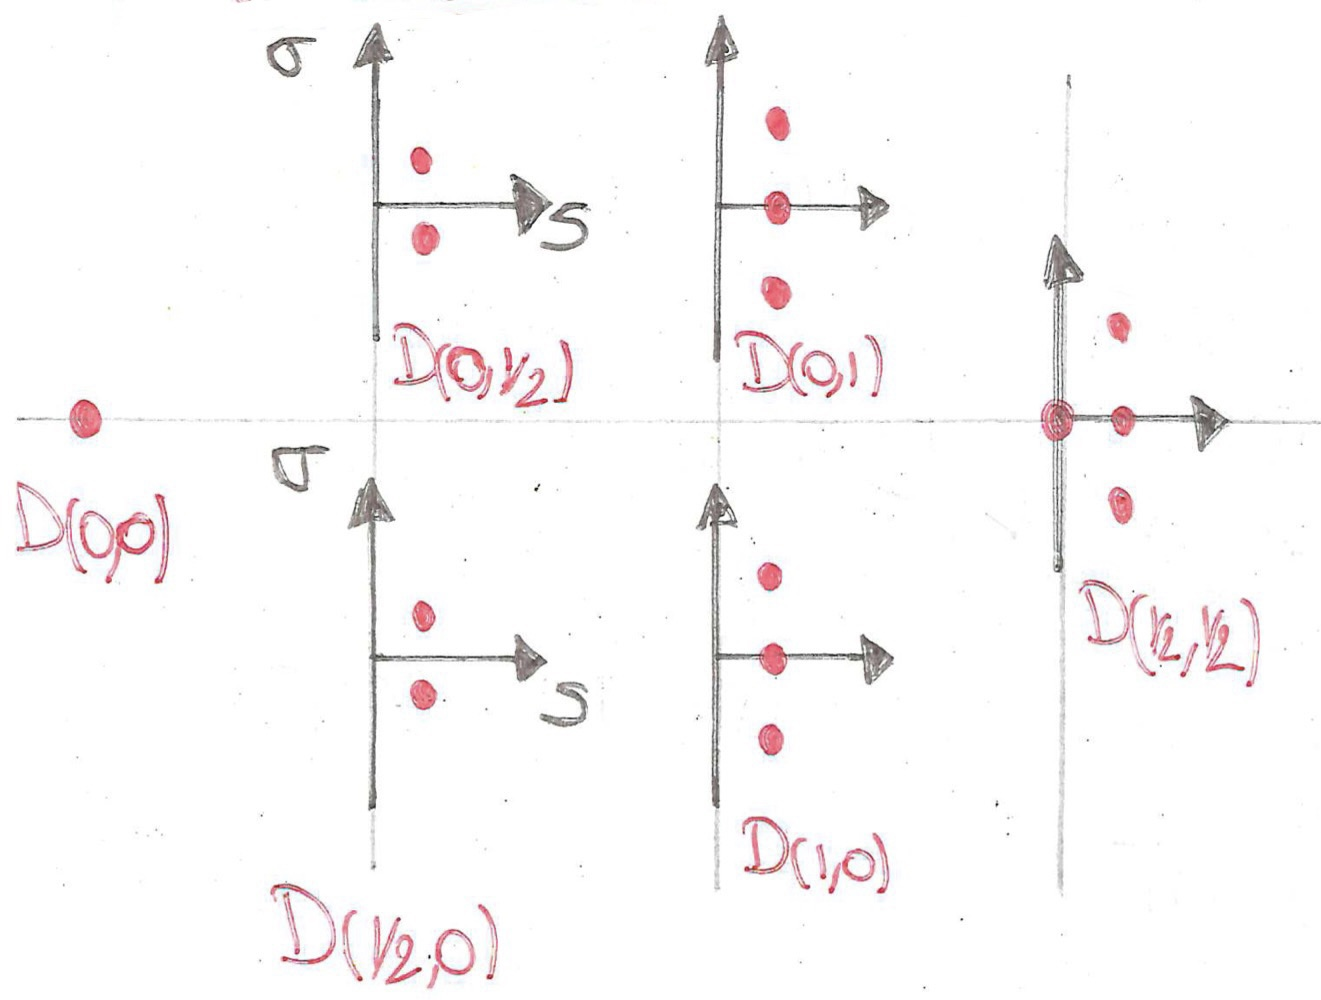
\includegraphics[]{images_ch7/repscheme.jpg}

\begin{example}
    \textbf{(Il campo di spin 1.)}

    Consideriamo il caso di un campo massivo con spin $s=1$. 

    Con riferimento al precedente schema, potremmo considerare la rappresentazione $(1,0)$ così come la $(0,1)$, in quanto entrambi contengono il multipletto con $s=1$. Tuttavia queste due rappresentazioni non sono invarianti sotto parità, per via del fatto che $\Vec{J}$ non cambia segno sotto parità, mentre $\Vec{K}$ si (intuitivamente perché la velocità cambia di segno sotto $\mathbb P$). Di conseguenza:
    \[
    \begin{aligned}
        \Vec{M} &= \frac{1}{2}(\Vec{J}+i\Vec{K}) \\
        \Vec{N} &= \frac{1}{2}(\Vec{J}-i\Vec{K})   
    \end{aligned}
    \quad
    \xrightarrow{\mathbb P}
    \quad
    \begin{aligned}
        \frac{1}{2}(\Vec{J}-i\Vec{K}) &= \Vec{N}\\
        \frac{1}{2}(\Vec{J}+i\Vec{K}) &= \Vec{M}   
    \end{aligned}
    \]
    Ovvero, in generale: $\boxed{(j_1,j_2)\xrightarrow{\mathbb P}(j_2,j_1)}$.

    Quello che stiamo dicendo è che in presenza della simmetria di parità, sia $(j_1,j_2)$ che $(j_2,j_1)$ dovrebbero essere presenti.

    Nel caso di nostro interesse, \textbf{la corretta identificazione è con la rappresentazione $\mathbf{\big(\frac{1}{2},\frac{1}{2}\big)}$, invariante sotto parità e contenente un solo multipletto con $\mathbf{s=1}$} e si può dimostrare che \textit{la rappresentazione ${\big(\frac{1}{2},\frac{1}{2}\big)}$ è equivalente alla rappresentazione 4-vettoriale del gruppo di Lorentz}.

    Intuitivamente questo si può capire considerando un 4-vettore $V^\mu = (V^0,\Vec{V})$ e notando che questo corrisponde ad una rappresentazione irriducibile del gruppo di Lorentz, in quanto una generica trasformazione di Lorentz mixa in generale tutte le componenti. 

    Se ci si restringe ad una trasformazione che sia una rotazione pura $\Lambda_R$, tuttavia, si trova che la componente temporale, non trasformando sotto rotazioni, ha spin $s=0$, mentre quella vettoriale trasforma, chiaramente, come un vettore ed hanno spin $s=1$.

    Abbiamo quindi \(V^\mu \xrightarrow[]{SO(3)}0\oplus1\), i.e. la rappresentazione 4-vettoriale si decompone in singoletto più tripletto di spin sotto $SO(3)$.
\end{example}

\section{Soluzione della Connessione $\pazocal P-\pazocal L$}

L'idea è quella di risolvere le equazioni (\ref{eq:poinc_lorentz_conn}) nel caso massless, che quindi ci permette di restare nella base di elicità. Lo faremo nel caso di un bosone vettore, come il fotone, ad esemplificare il caso dell'elettromagnetismo, ma la matematica che c'è dietro si può applicare anche al caso della gravità, in cui lo spin dell'ipotetico gravitone è 2.

\subsection{Bosone vettore massless}
Nel caso massless, le (\ref{eq:poinc_lorentz_conn}) si semplificano in accordo con la (\ref{eq:poincare_action_massless_genericstates}) e ci troviamo a dover risolvere il sistema:
\begin{equation}
    \begin{aligned}
        &e^{i\theta(\Lambda, p)\lambda} u^a(\Vec{p},\lambda) = 
        \big[\mathscr D(\Lambda^{-1})\big]^a_{~b}u^b(\Vec{p}_\Lambda,\lambda)\\
        &e^{-i\theta(\Lambda, p)\lambda} v^a(\Vec{p},\lambda) = \big[\mathscr D(\Lambda^{-1})\big]^a_{~b}v^b(\Vec{p}_\Lambda,\lambda)
    \end{aligned}
    \label{eq:poinc_lorentz_conn_massless}
\end{equation}

Ora invertiamo queste equazioni sfruttando il fatto che, in quanto rappresentazione, $\mathscr D(\Lambda^{-1}) = \mathscr D(\Lambda)^{-1}$ e che $\big[\mathscr D(\Lambda)\big]^c_{~a}\big[\mathscr D(\Lambda)^{-1}\big]^a_{~b} = \delta^c_b$. Con un paio di passaggi banali si arriva al sistema:
\begin{equation}
    \begin{aligned}
        &\big[\mathscr D(\Lambda)\big]^c_{~a} u^a(\Vec{p},\lambda) = 
        e^{-i\theta(\Lambda, p)\lambda}u^c(\Vec{p}_\Lambda,\lambda)\\
        &\big[\mathscr D(\Lambda)\big]^c_{~a} v^a(\Vec{p},\lambda) = e^{i\theta(\Lambda, p)\lambda}v^c(\Vec{p}_\Lambda,\lambda)
    \end{aligned}
    \label{eq:poinc_lorentz_conn_massless_inverted}
\end{equation}

Inoltre, stiamo considerando un campo 4-vettoriale massless, in cui gli spinori sono i vettori di polarizzazione, ovvero il campo:
\begin{equation}
    A^\mu(x) \equiv \sum_\lambda \int_{}\frac{d^3\Vec p}{(2\pi)^3\sqrt{2p^0}}\big[\varepsilon^\mu(\Vec{p},\lambda)a(\Vec{p},\lambda)e^{-ip\cdot x}+\varepsilon^\mu(\Vec{p},\lambda)^\ast a^\dagger(\Vec{p},\lambda)e^{ip\cdot x}\big]
    \label{eq:photon_field}
\end{equation}
le cui le due componenti sono legate dalla sola coniugazione di carica ed il sistema si riduce dunque ad una singola equazione da risolvere, valida $\forall~\Vec{p}$ e $\forall~\Lambda$. Se consideriamo la rappresentazione defining del gruppo di Lorentz, i.e. $\mathscr D(\Lambda) \equiv \Lambda$, abbiamo:

\begin{equation}
    \boxed{e^{-i\theta(\Lambda, p)\lambda}\varepsilon^\mu(\Vec{p}_\Lambda,\lambda) = \Lambda^\mu_{~\nu} \varepsilon^\nu(\Vec{p},\lambda)}
    \label{eq:poinc_lorentz_conn_massless_merged}
\end{equation}

La strategia di risoluzione è sostanzialmente la stessa che abbiamo delineato qualche pagina fa nel caso massivo, va solo riadattata con le giuste accortezze:
\begin{enumerate}
    \item[\textbf{1)}] Consideriamo il vettore di riferimento $p^\mu_\text{ref} = k(1,0,0,1)$, che implica $\Vec{p}_\text{ref} = k\hat{z}$, e consideriamo $\Lambda \rightarrow W\in \mathscr{G}(\Vec{p}_\text{ref}) = E(2)$, trasformazione che lascia il vettore di riferimento invariato e che quindi implica $p_\Lambda =\Lambda p_\text{ref} = p_\text{ref}$. Di conseguenza riscriviamo l'equazione:
    \begin{equation}
        \boxed{e^{-i\theta(W, p_\text{ref})\lambda}\varepsilon^\mu(\Vec{p}_\text{ref},\lambda) = W^\mu_{~\nu} \varepsilon^\nu(\Vec{p}_\text{ref},\lambda)}
        \label{eq:poinc_lorentz_conn_massless_merged_step1}
    \end{equation}
    Risolvendo questa equazione otteniamo $\varepsilon^\mu(\Vec{p}_\text{ref},\lambda)$.
    
    \item[\textbf{2)}] Noto $\varepsilon^\mu(\Vec{p}_\text{ref},\lambda)$, dobbiamo generalizzarlo al caso di impulso $\Vec{p}$ qualunque.

    Per farlo partiamo dalla (\ref{eq:poinc_lorentz_conn_massless_merged}) e scegliamo $\Lambda = H\big(\hat{p},\frac{|\Vec p|}{k}\big)^{-1}$ e seguendo la stessa logica del caso massivo, ma applicata alla fase invece che alla rotazione di Wigner, troviamo che:
    \[
    \theta(\Lambda = H^{-1}, p_\text{ref}) =  H\Big(\hat{p}_\Lambda,\frac{|\Vec p_\Lambda|}{k}\Big)^{-1}\underbrace{\Lambda H\Big(\hat{p},\frac{|\Vec p|}{k}\Big)}_{=\mathbb 1} = H\Big(\hat{p}_\Lambda,\frac{|\Vec p_\Lambda|}{k}\Big)^{-1}
    \]
    che riporta il vettore $\Vec p_\Lambda$ in $\Vec p_\text{ref}$. Ma da quanto appena visto $\Vec p_\Lambda =\Vec p_\text{ref}$, quindi $\theta(H^{-1}, p_\text{ref}) = \mathbb 1_{E(2)} = 0$.

    Ma allora possiamo beneficiare di una drastica semplificazione della (\ref{eq:poinc_lorentz_conn_massless_merged}), che difatti si riscrive:
    \begin{equation}
    \boxed{ \varepsilon^\mu(\Vec{p},\lambda)= H\Big(\hat{p},\frac{|\Vec p|}{k}\Big)^\mu_{~\nu}\varepsilon^\nu(\Vec{p}_\text{ref},\lambda)}
    \label{eq:poinc_lorentz_conn_massless_merged_step2}
\end{equation}
\end{enumerate}

Tutto sembra filare liscio fin qui, eppure c'è un piccolo problema (in realtà tutt'altro che piccolo), ma arriviamoci per gradi. \textbf{Partendo dallo step 1)}, l'equazione (\ref{eq:poinc_lorentz_conn_massless_merged_step1}) vale per ogni elemento $W$ del gruppo piccolo di $\Vec p_\text{ref}$, ovvero $E(2)$ in cui abbiamo due scelte naturali per $W$: una rotazione attorno a $\hat z$ o una traslazione nello spazio Euclideo.

\begin{enumerate}
    \item[\textbf{a)}] \textbf{$\mathbf{W}$ è una rotazione attorno $\hat{\mathbf{z}}$.}

    In questo caso, come già fatto più volte, possiamo sfruttare la proprietà della fase di Wigner che ci garantisce la sua uguaglianza con l'angolo di rotazione $\phi$ attorno a $\hat z$. Abbiamo quindi, esplicitando l'elicità, che nel caso di un bosone vettore massless assume i valori $\lambda=\pm 1$:
    \begin{align*}
        &e^{\mp i\phi}\varepsilon^\mu(k\hat z,\pm 1) = W(\phi)^\mu_{~\nu} \varepsilon^\nu(k\hat z,\pm 1) \\
        &\text{con } W(\phi) =
        \begin{pmatrix}
            \begin{array}{cccc}
                1 & 0 & 0 & 0 \\
                0 & \cos\phi & -\sin\phi & 0 \\
                0 & \sin\phi & \cos\phi & 0 \\
                0 & 0 & 0 & 1
            \end{array}
        \end{pmatrix}
    \end{align*}
    Svolgendo esplicitamente i conti, troviamo senza troppa difficoltà che per $\mu=0$ e $\mu=3$, essendo $\phi$ generico, deve valere:
    \[
    \boxed{\varepsilon^0(k\hat z,\pm 1) = \varepsilon^3(k\hat z,\pm 1)\overset{!}{=} 0}
    \]
    Questa equazione ci sta dicendo che dei quattro gradi di libertà equivalenti alle quattro equazioni del sistema, due sono automaticamente soppressi, il che è totalmente consistente con il fatto che dal punto di vista del gruppo di Poincaré un bosone vettore massless (come il fotone) ha due soli gradi di libertà (i suoi stati di elicità).

    Dalle altre due componenti ($\mu=1$ e $\mu=2$) otteniamo il seguente sistema:
    \[
    \begin{cases}
        e^{\mp i\phi}\varepsilon^1(k\hat z,\pm 1) = \cos\phi\varepsilon^1(k\hat z,\pm 1) -\sin\phi \varepsilon^2(k\hat z,\pm 1)\\
        e^{\mp i\phi}\varepsilon^2(k\hat z,\pm 1) = \sin\phi\varepsilon^1(k\hat z,\pm 1) + \cos\phi \varepsilon^2(k\hat z,\pm 1)
    \end{cases}
    \]
    ed esplicitando, per mezzo della formula di Eulero, $e^{\mp i\phi}=\cos\phi \mp i\sin\phi$ questo si riduce ad una singola equazione: \marginnote{\textbf{Attenzione:} il segno $\mp$ davanti ad $\varepsilon^1$ corrisponde al caso in cui $\lambda=\pm 1$ rispettivamente, come conseguenza del fatto che l'esponenziale ha il segno “$-$” all'esponente.}
    \[
    \boxed{\mp i\varepsilon^1(k\hat z,\pm 1) = -\varepsilon^2(k\hat z,\pm 1)}
    \]
    Se prendiamo la cosiddetta convenzione di “polarizzazione circolare”, i.e. scegliamo $\varepsilon^1(k\hat z,\pm 1) \equiv \frac{1}{\sqrt{2}}$ troviamo che:
    \begin{equation}
        \boxed{\varepsilon^\mu(k\hat z, +1) = \frac{1}{\sqrt{2}}
        \begin{pmatrix}
            \begin{array}{c}
                0  \\
                1  \\
                i  \\
                0
            \end{array}    
        \end{pmatrix} \quad
        \varepsilon^\mu(k\hat z,- 1) = \frac{1}{\sqrt{2}}
        \begin{pmatrix}
            \begin{array}{c}
                0  \\
                1  \\
                -i  \\
                0
            \end{array}    
        \end{pmatrix}}
        \label{eq:polvects_circ_pol_choice}
    \end{equation}

    \item[\textbf{b)}] \textbf{$\mathbf{W}$ è una traslazione nello spazio Euclideo.}
    
    Un elemento del gruppo piccolo di questo tipo può essere scritto genericamente come:
    \[
    W = \exp \big( -i\alpha T_x -i\beta T_y \big) ~,\quad \alpha,\beta \in\mathbb R
    \]
    con $T_x\equiv J_\text{vec}^1 + K_\text{vec}^2$ e $T_y\equiv J_\text{vec}^2 - K_\text{vec}^1$.

    In questo caso la fase di Wigner è $\textcolor{blue}{\theta (W, p_\text{ref})=0}$, intuitivamente poiché essa “misura” la componente $J^3$ che in questo caso non figura, non essendo $W$ una rotazione attorno a $\hat{z}$.

    Troviamo quindi l'equazione:
    \begin{align*}
        \underbrace{e^{-i\theta(W, p_\text{ref})\lambda}}_{\textcolor{blue}{=1}}\varepsilon^\mu(k\hat{z}, \lambda) &= \big[ \exp\big( -i\alpha T_x -i\beta T_y \big)\big]^{\mu}_{~\nu}\varepsilon^\nu(k\hat{z}, \lambda) =\\
        &=\begin{pmatrix}
            \begin{array}{cccc}
               1+\frac{\alpha^2+\beta^2}{2}  & -\beta  & \alpha  & -\frac{1}{2}(\alpha^2+\beta^2) \\
               -\beta  &  1  &  0  & \beta \\
               \alpha  &  0  &  1  & -\alpha \\
                \frac{1}{2}(\alpha^2+\beta^2) & -\beta & \alpha  &  1-\frac{\alpha^2+\beta^2}{2}
            \end{array}
        \end{pmatrix}
        \begin{pmatrix}
            \begin{array}{c}
                0 \\
                1 \\
                \lambda i\\
                0
            \end{array}
        \end{pmatrix}
    \end{align*}
    dove il calcolo dell'esponenziale di matrice è stato fatto con \href{https://www.wolfram.com/mathematica/}{Mathematica} e si è sostituita l'espressione dei vettori di polarizzazione nel caso della polarizzazione circolare.

    Se ora svolgiamo il prodotto, troviamo il seguente risultato:
    \begin{equation}
        \boxed{\varepsilon^\mu(k\hat{z}, \pm 1) = \frac{1}{\sqrt{2}}
        \begin{pmatrix}
            \begin{array}{c}
                -\beta\pm i\alpha \\
                1 \\
                \pm i\\
                -\beta\pm i\alpha
            \end{array}
        \end{pmatrix} = \varepsilon^\mu(k\hat{z}, \pm 1) + \frac{-\beta\pm i\alpha}{\sqrt{2}k}p^\mu_\text{ref}}
        \label{eq:inconsistency}
    \end{equation}
    
    Ma se guardiamo bene, ci accorgiamo della presenza di un'inconsistenza, quella che abbiamo annunciato poco sopra. Infatti, questa equazione richiede che $-\beta\pm i\alpha =0$, ovvero $\beta = \pm i\alpha$, ma $\alpha$ e $\beta$ sono reali, ergo \textbf{questa condizione non può essere verificata in nessun caso!}
\end{enumerate}

Il problema che abbiamo incontrato risiede nel fatto che, in termini tecnici,\textit{ i vettori di polarizzazione appartengono ad una rappresentazione di }$\mathscr G(\Vec p_\text{ref})$ \textit{differente da quella a cui invece appartengono gli stati particellari che dovrebbero descrivere!} Infatti, mentre gli stati particellari sono invarianti sotto traslazioni Euclidee, i.e.:
\begin{align*}
    &T_x|0, k\hat{z}, \lambda\rangle = T_y|0, k\hat{z}, \lambda\rangle = 0 \\
    &\Rightarrow e^{-i\alpha T_x -i\beta T_y}|0, k\hat{z}, \lambda\rangle = |0, k\hat{z}, \lambda\rangle
\end{align*}
troviamo che l'azione di $W^{\mu}_{~\nu}$ (traslazione Euclidea) sui vettori dei polarizzazione è assimilabile ad una sorta di trasformazione di Gauge, che produce uno shift dal vettore di partenza di un termine proporzionale a $p^\mu$.

In altre parole quello che abbiamo sbagliato è stato assumere che il campo $A^\mu$ (e di conseguenza i vettori di polarizzazione) trasformasse come un 4-vettore sotto trasformazioni di Lorentz, in quanto questo non è vero!

\begin{exercise}
    Calcolare esplicitamente la struttura della legge di trasformazione di $\varepsilon^\mu(\Vec{p}, \lambda)$ sotto una generica trasformazione di Lorentz. \textbf{[Conti svolti Lezione 28 pag.39÷40]}

    \textbf{Soluzione. } 
    \begin{equation}
        \boxed{\Lambda^\mu_{~\nu}\varepsilon^\nu(\Vec{p}, \lambda) = e^{-i\theta\lambda}\varepsilon^\mu(\Vec{p}, \lambda) + e^{-i\theta\lambda}\frac{(-\beta+i\alpha\lambda)}{\sqrt{2}k}(\Lambda p)^\mu}
        \label{eq:generic_lorentztransform_polvec}
    \end{equation}
    L'equazione (\ref{eq:generic_lorentztransform_polvec}) può essere riscritta come segue, evidenziando la similitudine con le trasformazioni di gauge:
    \begin{equation}
        \boxed{e^{i\theta\lambda}\varepsilon^\mu(\Vec{p}, \lambda) = (\Lambda^{-1})^\mu_{~\nu}\varepsilon^\nu(\Vec{p}, \lambda) +\frac{(-\beta+i\alpha\lambda)}{\sqrt{2}k} p^\mu}
        \label{eq:generic_lorentztransform_polvec_inv}
    \end{equation}
\end{exercise}
\subsubsection{Interpretazione e Conseguenze}
Abbiamo scoperto che la connessione particella-campo non ha soluzione nel caso di una particella massless di spin 1 e che, in particolare, questo è dovuto all'errata assunzione che $A^\mu(x)$ trasformi come un 4-vettore sotto trasformazioni di Lorentz.

\begin{exercise}
    Calcolare esplicitamente la struttura della legge di trasformazione di $A^\mu(x)$ (\ref{eq:photon_field}) sotto una generica trasformazione di Lorentz, i.e. $U(\Lambda)A^\mu(x)U(\Lambda)^{-1}$. \textbf{[Conti svolti Lezione 28 pag. 40÷42]}

    \textbf{Soluzione. } 
    I passaggi sono piuttosto banali, si tratta di utilizzare le proprietà di trasformazione degli operatori di creazione e distruzione (\ref{eq:creation_operators_underpoincare}) e (\ref{eq:annihil_operators_underpoincare}), la proprietà di trasformazione del vettore di polarizzazione scritta nella forma (\ref{eq:generic_lorentztransform_polvec_inv}) e di ridefinire il termine proporzionale a $p^\mu$ con la derivata rispetto ad $x_\mu$ di una generica funzione $\Omega_\Lambda(x)$ in cui $x_\mu p^\mu$ figura come argomento di un esponenziale (in modo che la derivata riproduca la proporzionalità corretta).

    In definitiva si trova
    \begin{equation}
        \boxed{
        U(\Lambda)A^\mu(x)U(\Lambda)^{-1} = \Lambda^\mu_{~\nu} A^\nu(\Lambda x) + \partial^\mu \Omega_\Lambda(x)
        }
        \label{eq:generic_poincaretransform_photonfield}
    \end{equation}
    Come anticipato, il campo quantistico che dovrebbe descrivere il fotone non trasforma in maniera covariante sotto Lorentz, i.e. non è un 4-vettore.
\end{exercise}
Possiamo quindi affermare quanto segue:
\begin{enumerate}
    \item[\textbf{i)}] Siccome l'operatore di campo associato al fotone non trasforma in maniera covariante sotto trasformazioni di Lorentz, non possiamo inserirlo in una densità di Lagrangiana e sperare di ottenere una teoria realmente invariante sotto Lorentz. La teoria in questo caso sarebbe solo apparentemente invariante!
    \item[\textbf{ii)}] Se la teoria fosse invariante sotto la sostituzione formale (traformazione di gauge) $A_\mu\rightarrow A_\mu + \partial_\mu\lambda(x)$ per una generica funzione $\lambda(x)$, allora il pezzo extra che emerge dalla trasformazione di Lorentz sarebbe innocuo. L'invarianza sotto tale sostituzione formale è detta \textbf{invarianza di gauge}.
    
    Ci sono due possibili implementazioni dell'idea al punto ii):
    \begin{itemize}
        \item Consideriamo il \textit{tensore di Faraday:} $F^{\mu\nu} = \partial^\mu A^\nu - \partial^\nu A^\mu$. Questo tensore è invariante sotto trasformazioni di gauge, i.e. \textit{è un invariante di gauge} e ciò significa che $F^{\mu\nu}$ è un vero tensore e trasforma come un tensore:
        \[
        \boxed{U(\Lambda)F^{\mu\nu}(x)U(\Lambda)^{-1} = (\Lambda^{-1})^\mu_{~\rho}(\Lambda^{-1})^\nu_{~\sigma}F^{\rho\sigma}(\Lambda x)}
        \]
        possiamo quindi utilizzare $F_{\mu\nu}$ per costruire quantità che siano invarianti di Lorentz, e.g. $F_{\mu\nu}F^{\mu\nu}$, $F_{\mu\nu}\bar\psi \sigma^{\mu\nu}\psi$, ...
    
        Tuttavia \textbf{non è così che funziona la natura} e c'è un motivo se continuiamo ad utilizzare $A^\mu$ nella Lagrangiana. Inoltre la legge di Coulomb si può derivare solo dall'interazione $A_{\mu}\bar\psi \gamma^{\mu}\psi$ e non da $F_{\mu\nu}\bar\psi \sigma^{\mu\nu}\psi$, e questo è dovuto al fatto che in quest'ultima appare un impulso dalle regole di Feynman e ciò non ci consente di generare un'interazione a lungo raggio. Inoltre $F_{\mu\nu}\bar\psi \sigma^{\mu\nu}\psi$ è anche non rinormalizzabile, in quanto il coupling avrebbe una dimensione di massa negativa!
    
        \item Accoppiamo $A_\mu$ ad una corrente conservata $j^\mu$ (t.c. $\partial_\mu j^\mu = 0$ e tale da essere un vero 4-vettore, ossia da trasformare come 4-vettore).

        Possiamo farlo in quanto considerando l'accoppiamento $A_\mu j^\mu$, questo è invariante a vista, ma è anche invariante sotto trasformazioni di gauge! Infatti:
        \[
        A_\mu j^\mu \rightarrow A_\mu j^\mu + (\partial_\mu\lambda)j^\mu \overset{[...]}{=} A_\mu j^\mu - \lambda\Ccancel[Black]{(\partial_\mu j^\mu)} = A_\mu j^\mu 
        \]

        Va tuttavia sottolineato il fatto che questa procedura sia un po' tricky da implementare in una teoria di campo generica, in quanto dal teorema di Noether sappiamo che le correnti si conservano solo sulla shell di massa, ma \textbf{questa è la strada che la natura ha scelto di seguire}.
    \end{itemize}

    \item[\textbf{iii)}] L'origine dell'invarianza di gauge è la seguente: se vogliamo descrivere una particella massless di spin 1 con un campo quantistico $A^\mu(x)$, allora la teoria risultante è invariante sotto trasformazioni di Lorentz \textbf{SOLO} se imponiamo l'invarianza di gauge!
    
    \item[\textbf{iv)}] \textbf{L'invarianza di gauge non è un simmetria} dal punto di vista fisico, in quanto non è associata a nessuna trasformazione nello spazio di Hilbert della particella. 

    Anzi, a dirla tutta \textbf{è proprio l'opposto}: l'invarianza di gauge è conseguenza della nostra ostinazione nel voler descrivere un bosone vettore massless con un campo quantistico, è una ridondanza che emerge dal fatto che abbiamo una classe di trasformazioni sotto le quali gli operatori di campo trasformano, ma non gli stati, i.e. le traslazioni Euclidee! Abbiamo infatti:

    \[
    \begin{aligned}
        &|0, k\hat{z}, \lambda\rangle \\ 
        T_x&|0, k\hat{z}, \lambda\rangle = 0\\
        T_y&|0, k\hat{z}, \lambda\rangle = 0
    \end{aligned}
    \quad\leftrightarrow\quad
    \begin{aligned}
        &\varepsilon^\mu(k\hat{z}, \lambda)\\ 
        W^\mu_{~\nu}&\varepsilon^\mu(k\hat{z}, \lambda) \overset{(\ref{eq:inconsistency})}{=} \varepsilon^\mu(k\hat{z}, \lambda) + \frac{(-\beta+i\alpha\lambda)}{\sqrt{2}k}p^\mu_\text{ref}
    \end{aligned}
    \]
    A questo punto possiamo finalmente generalizzare la (\ref{eq:inconsistency}) ad impulso generico, svolgendo sostanzialmente lo step 2, tramite la (\ref{eq:poinc_lorentz_conn_massless_merged_step2}):
    \begin{align*}
         \varepsilon^\mu(\Vec{p},\lambda) &= H\Big(\hat{p},\frac{|\Vec p|}{k}\Big)^\mu_{~\nu}\varepsilon^\nu(k\hat{z}, \lambda) + \frac{(-\beta+i\alpha\lambda)}{\sqrt{2}k}H\Big(\hat{p},\frac{|\Vec p|}{k}\Big)^\mu_{~\nu}p^\nu_\text{ref}\\
         &= \varepsilon^\mu(\Vec{p},\lambda) +\underbrace{\frac{(-\beta+i\alpha\lambda)}{\sqrt{2}k}}_{\equiv C_\lambda}p^\mu
    \end{align*}
    
    Ottenendo in definitiva\footnote{Notare come questa equazione giustifichi la sostituzione fatta per ottenere la (\ref{eq:ward_id_vertex})}:
    \begin{equation}
         \boxed{\varepsilon^\mu(\Vec{p},\lambda) = \varepsilon^\mu(\Vec{p},\lambda) + C_\lambda p^\mu}
         \label{eq:generalized_polvec}
    \end{equation}
    
    Entrambi i membri dell'equazione devono descrivere lo stesso fotone fisico, ma abbiamo ancora un pezzo in più nel RHS. Tuttavia, al momento del calcolo di una generica ampiezza $\mathscr M_\mu$, avremo sempre:
    \[
    \varepsilon^\mu(\Vec{p},\lambda)\mathscr M_\mu = \big(\varepsilon^\mu(\Vec{p},\lambda) + C_\lambda p^\mu\big)\mathscr M_\mu
    \]
    ma sappiamo benissimo che $\boxed{p^\mu \mathscr M_\mu = 0}$, ce lo garantisce l'identità di Ward (\ref{eq:WT_ID_Nphotons}), che segue direttamente dall'accoppiamento di $A^\mu$ con una corrente conservata!
\end{enumerate}


\end{document}
% 
\begin{figure}[h]
    \centering
    \includegraphics{images/semplicementepanati.png}
    \caption*{}
    \label{fig:my_label}
\end{figure}
